\chapter{绪论}
%
\section{研究背景和意义}
% \subsection{研究背景和意义}
%
2024年也被称为低空经济元年,全国两会首次将“低空经济”写入政府工作报告中。12月23日,教育部公示北京航空航天大学等6所高校申请增设“低空技术与工程”新专业。12月25日,国家发改委挂牌成立低空经济司。种种迹象表明低空经济这一战略新兴产业具有广阔的发展前景,得到了各界的重视。无人机(Unmanned Aerial Vehicle,UAV)作为低空经济的重要形态之一,近些年来发展得如火如荼,已经在军事、民用、科研等领域得到了广泛应用。顾名思义,无人机是一种不需要飞行员在飞机上驾驶的飞行器,它的飞行控制可以由飞行员在地面的控制站上进行操纵,也可以基于事先设计好的轨迹完全自主飞行,或者借助如人工智能(Artificial Intelligence,AI)等先进技术在复杂环境中实时地规划轨迹来避障飞行\cite{rezwanArtificialIntelligenceApproaches2022}。

无人机最早于第一次世界大战期间被研制出来用于军事对抗。受限于二十世纪初的科学技术条件,当时的无人机并没有在战场上发挥很大的作用,但是人们并没有因此停止对无人机的研究与发展。时至今日,无人机在俄乌战争中被大规模使用,主要用来执行目标搜寻、侦察、打击和救援等任务,深刻地影响了战场局势。在2022年的最后一个晚上,乌克兰的四旋翼无人机向俄罗斯士兵投下了小型炸弹,其凭借着机载的热成像系统实现了在漆黑的夜晚对俄罗斯士兵进行准确打击\cite{kunertovaWarUkraineShows2023}。无独有偶,由俄罗斯Kronshtadt公司开发的“猎户座(Orion)”固定翼无人机(见图\ref{Orion})也已成功用于攻击乌克兰阵地。该无人机前部安装了一个可以转动的炮塔系统,内部装有红外传感器和激光雷达等设备,用于引导高精武器准确打击目标。除军事用途外,无人机也在民用领域大展身手。例如,无人机结合人工智能以及机器学习(Machine Learning,ML)方法,通过提升效率、环境可持续性和数据驱动的决策指定,为精准农业带来了重大革新\cite{agrawal2024transforming}。2022年,意大利Cristiano Fragassa教授团队利用无人机从不同的飞行高度拍摄杂草丛生的田地的图像,开发和测试了一种机器学习方法用来识别植被斑块。该方法可以精确地识别出整个大规模耕作田中的农作物和杂草,该信息可以用来帮助减少水、肥料和除草剂的使用\cite{fragassaNewProcedureCombining2023}。在国内,以大疆创新和极飞科技等为代表的科技公司都有自研的农业无人机产品。以极飞P150PRO 2025款农业无人机为例(见图\ref{P150PRO}),该无人机集农药喷洒、种子播撒、货物运输和航拍测绘多种功能为一体,每分钟最大喷洒流量可达32升,单次航测面积最大可达300亩。科研院校中如中国农业大学、华南农业大学\cite{liuAgriculturalUAVObstacle2024a}等也都在农业无人机方面取得研究进展。

\begin{figure}[htbp]
	\centering
	\begin{minipage}[c]{0.5\textwidth} % minipage将页面划分为0.5\textwidth
		\centering
		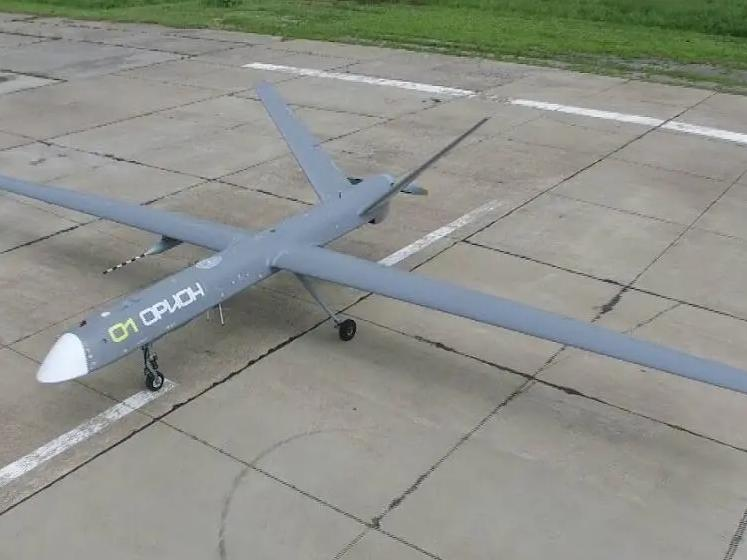
\includegraphics[width=6cm,height=5cm]{Fig/Orion.jpg}
		\caption{\label{Orion}猎户座固定翼无人机}
	\end{minipage}%
	\begin{minipage}[c]{0.5\textwidth}
		\centering
		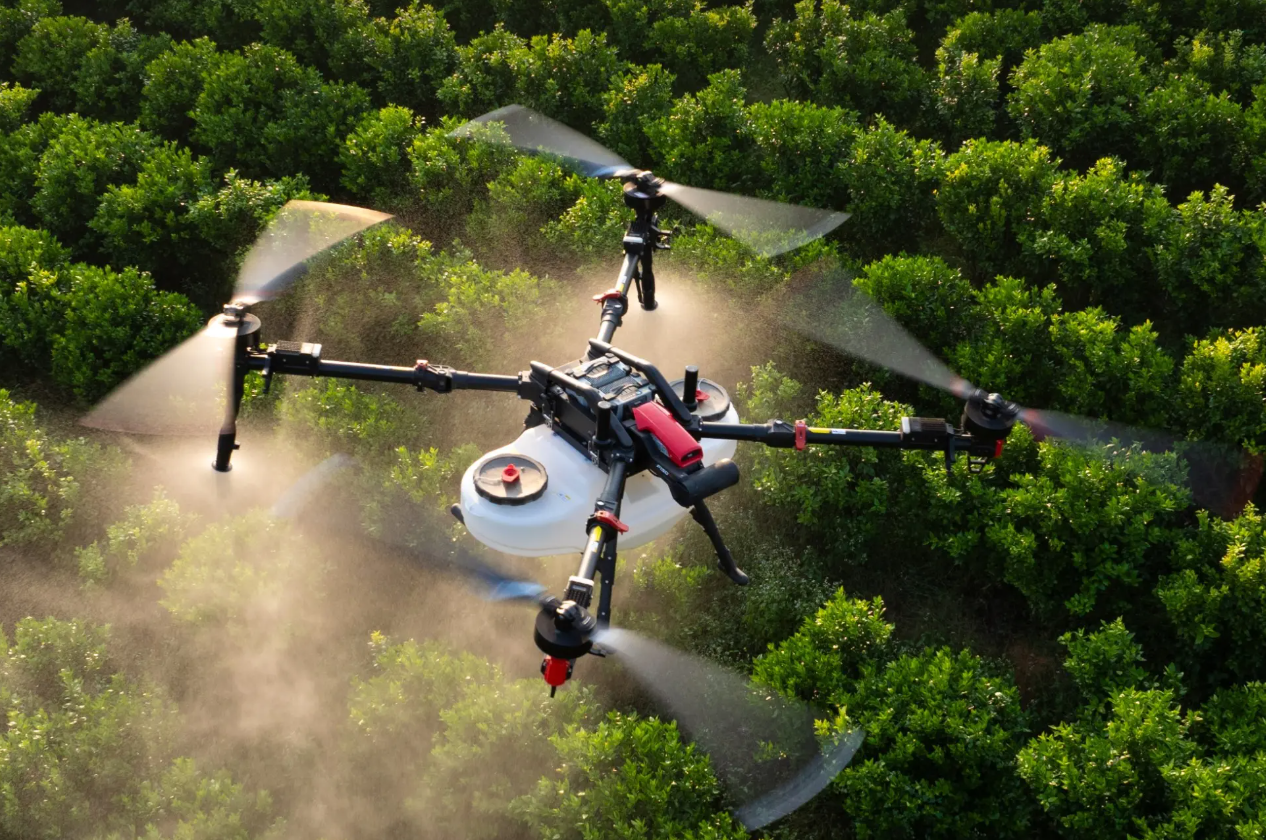
\includegraphics[width=7cm,height=5cm]{Fig/P150PRO.png}
		\caption{\label{P150PRO}极飞P150PRO农业无人机}
	\end{minipage}
\end{figure}

无人机发展百年,种类繁多,不同的任务需求驱动着创造不同类型的无人机。因此按照无人机的任务能力,可将其分为水平起飞着陆(Horizontal Take-off Landing,HTOL)、垂直起飞着陆(Vertical Take-off Landing,VTOL)、混合模型(倾转翼、倾转旋翼和涵道风扇)、直升机和非常规类型\cite{hassanalianClassificationsApplicationsDesign2017}。其中,涵道风扇无人机(Ducted Fan UAV,DFUAV)是指其螺旋桨被封闭在涵道内部的无人机,这些螺旋桨也被称为“风扇”,同时风扇滑流中安装有若干控制舵面进行控制。DFUAV既有旋翼无人机般的垂直起降能力,又可以像固定翼无人机那样高速巡航,而且这种特殊的配置结构具有空气动力效率高和操作安全性的优势\cite{johnsonModelingControlFlight2006b,choiStaticAnalysisSmall2012,zhangReviewDuctedFans2020b,qianImprovingPerformanceDucted2022,manzoor2022flight}。但不如人意的是,与开放旋翼相比,涵道风扇的罩状旋翼在飞行器周围的流场中会表现出强烈的耦合效应\cite{iiiNondimensionalModelingDuctedFan2012},并且由于其特殊的气动布局,DFUAV在垂直起降和水平巡航这两种不同的飞行模式下气动特性也完全不同\cite{johnsonModelingControlFlight2006b},这都对DFUAV的控制器设计提出了挑战。此外,针对DFUAV的轨迹规划的研究相对匮乏,这种研究的不足在一定程度上限制了DFUAV在复杂环境中的高效运作,不利于DFUAV的进一步推广应用。

正因如此,设计出适用于DFUAV的控制策略以及合理的轨迹规划方法,对于DFUAV的进一步发展具有重要意义。

\section{国内外研究现状}

\subsection{涵道风扇无人机}

目前已知的关于涵道风扇无人机的起源最早可以追溯到二十世纪三十年代,由意大利的Stipa和德国的Kort率先在该领域开展研究\cite{iiiNondimensionalModelingDuctedFan2012}。在二十世纪五十年代,美国宇航局在研究Doak VZ-4和Bell X-22涵道风扇垂直起降飞行器时投入了大量精力后取得一些进展,然而他们也发现了一些意料之外的特性,如从悬停到前飞过渡时,会出现机头上仰的趋势\cite{cookSummaryLiftLift1993}。Pereira等人\cite{pereiraHoverWindtunnelTesting2008}已经对涵道风扇早期的研究进行了详尽的回顾。近年来,随着先进的控制方法的提出和涵道风扇理论的进一步完善,涵道风扇无人机这一领域不仅引起了众多科研机构的广泛关注,还催生出了一系列具有里程碑意义的创新产品。

在二十世纪八十年代末期,美国Sikorsky航空公司试飞了一种名为“Cypher”的小型无人机。该无人机涵道直径1.75m,重量为20kg,采用共轴双桨结构提供动力,环形护罩在提升了拉力效率的同时也提升了其安全性。1992年4月,在初代Cypher的基础上,Cypher II进行了首次飞行。相比初代Cypher,Cypher II涵道直径1.9m,重量为110kg,并且在环形护罩外扩展了固定翼结构,并且尾部还有一个推进式螺旋桨,有效提升了Cypher II的飞行速度以及续航时间\cite{murphy1996air},最高时速可达230km/h,航程超过185km。

\begin{figure}[htbp]
	\centering
	\begin{minipage}[c]{0.5\textwidth} % minipage将页面划分为0.5\textwidth
		\centering
		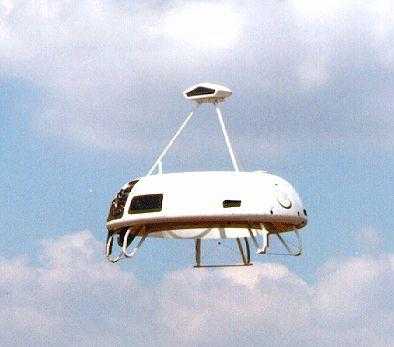
\includegraphics[width=6cm,height=5cm]{Fig/Cypher.jpg}
		\caption{\label{Cypher}Cypher}
	\end{minipage}%
	\begin{minipage}[c]{0.5\textwidth}
		\centering
		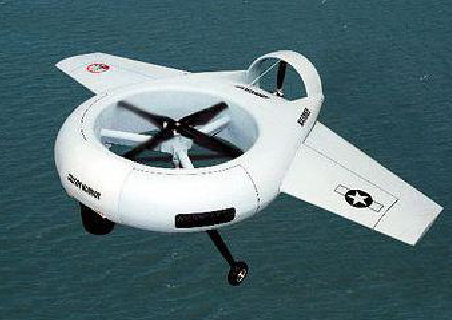
\includegraphics[width=6cm,height=5cm]{Fig/Cypher II.png}
		\caption{\label{Cypher II}Cypher II}
	\end{minipage}
\end{figure}

2003年,美国极光飞行科技公司根据国防高级研究计划局的“秘密无人机”计划开发了GoldenEye-100无人机,可垂直起降并且能携带11kg的有效载荷。次年7月,由GoldenEye-100衍生出的更小的GoldenEye-50无人机首飞。GoldenEye-50长70cm,翼展1.4m,最大飞行速度可达280km/h\cite{schaeferGoldenEyeClandestineUAV},并且在2005年4月进行了第一次自主水平飞行转换。GoldenEye-80是GoldenEye系列的第三个版本,长165cm,重达68kg,携带有高分辨率摄像机和激光测距仪等传感设备,设计意图用于满足美国陆军未来作战系统计划的要求。

2003年,Honeywell航空航天公司为美国陆军开发制造了RQ-16 T-Hawk微型无人机,并于2007年部署在了伊拉克战场上\cite{white2010upgrades}。该款无人机采用涵道风扇设计,涵道直径为35.5cm,总机重量为7.7kg,巡航速度可达74km/h,在战场上被广泛应用于可疑目标检查和跟随等任务。在2011年日本地震引发海啸进而导致核泄露后,4架T-Hawk被部署在福岛1号核电站,其机载的高分辨率摄像头拍摄了核电站受损部分的图像用于帮助日本核工程专家快速定位和解决问题。但是后来有两架T-Hawk在核反应堆上空坠毁,Honeywell公司并没有给出具体原因。

\begin{figure}[htbp]
	\centering
	\begin{minipage}[c]{0.5\textwidth} % minipage将页面划分为0.5\textwidth
		\centering
		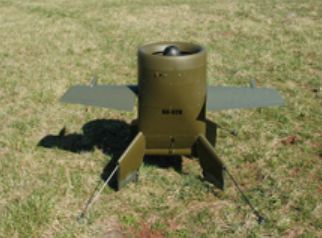
\includegraphics[width=6cm,height=5cm]{Fig/GoldenEye.png}
		\caption{\label{GoldenEye}GoldenEye}
	\end{minipage}%
	\begin{minipage}[c]{0.5\textwidth}
		\centering
		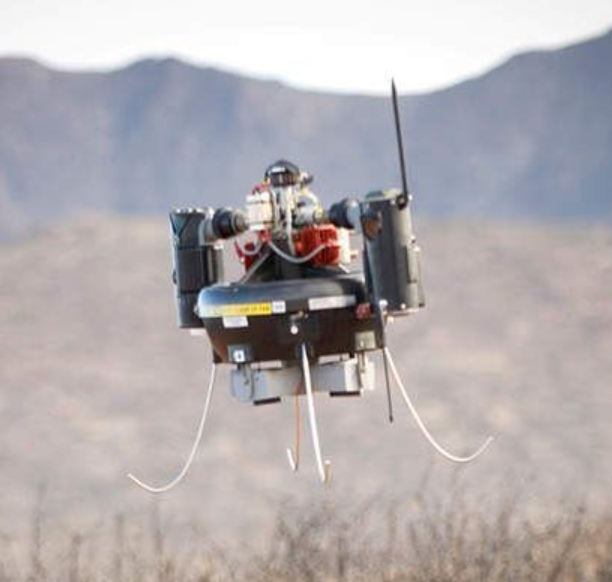
\includegraphics[width=6cm,height=5cm]{Fig/T-Hawk.png}
		\caption{\label{T-Hawk}T-Hawk}
	\end{minipage}
\end{figure}

2015年12月30日,由以色列Tactical Robotics公司研发的AirMule救护无人机首航。如图\ref{AirMule}所示,AirMule的起飞旋翼设置在了机身内部,由涵道壁包裹,尾部还有两个推进涵道风扇用于控制姿态。这种构型专为直升机不方便起降的情形而设计,如山川、林地等地形复杂的区域。由于AirMule可负载80kg的载重能力和150km/h的最大速度\cite{yuTechnicalAnalysisVTOL2016},未来还将用于运输货物等任务。

% \begin{figure}[htbp]
% 	\centering
% 	\begin{minipage}[c]{0.5\textwidth} % minipage将页面划分为0.5\textwidth
% 		\centering
% 		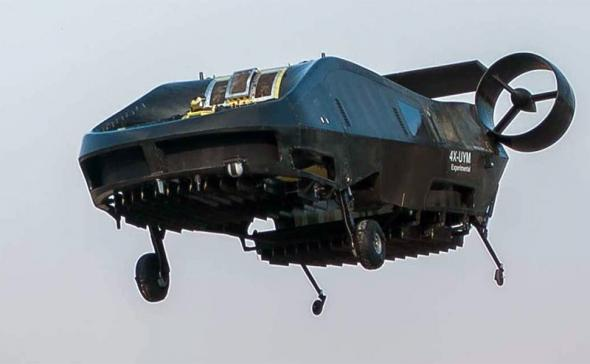
\includegraphics[width=7cm,height=5cm]{Fig/AirMule.jpg}
% 		\caption{\label{AirMule}AirMule}
% 	\end{minipage}%
% 	\begin{minipage}[c]{0.5\textwidth}
% 		\centering
% 		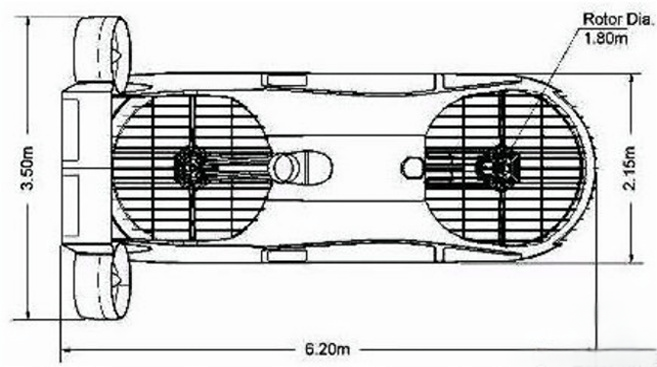
\includegraphics[width=7cm,height=5cm]{Fig/Airmule内部结构.png}
% 		\caption{\label{AirMule2}Airmule内部结构}
% 	\end{minipage}
% \end{figure}

\begin{figure}[htbp]
	\centering
    \subfloat[AirMule无人机]
		{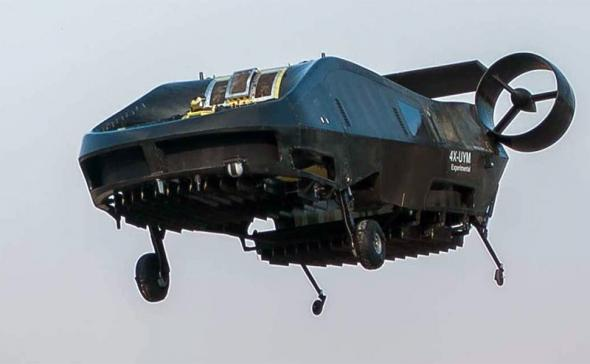
\includegraphics[width=7cm,height=5cm]{Fig/AirMule.jpg}
		\label{AirMule1}}
        \subfloat[AirMule内部结构]{
		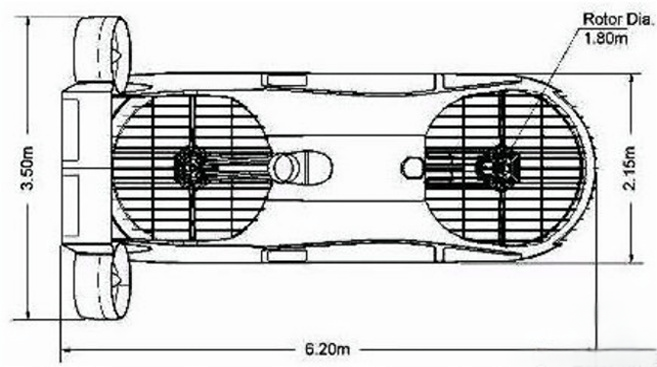
\includegraphics[width=7cm,height=5cm]{Fig/Airmule内部结构.png}
		\label{AirMule2}}
        \caption{AirMule无人机及内部结构}\label{AirMule}
\end{figure}

在2016年的HWTrek全球智能硬件创新与制造大会上,来自比利时无人机Fleye引发众人关注,如图所示。因其大小与篮球相当,许多媒体也把它称为“球形无人机”。Fleye也属于DFUAV的一种,摄像头安装在上部,下部为光流传感器,由于其安全小巧的特点,媒体预测其未来将会应用于室内摄影、娱乐等场合。除上述提到的采用涵道构型无人机外,还有由新加坡ST Aerospace研发的FanTail系列\cite{mateosanguinoDesignStabilizationCoanda2024}、Aesir公司的Odin\cite{crivoi2013survey}和美国联合宇航公司的iSTAR\cite{flemingImprovingControlSystem,lipera2001micro}等。

\begin{figure}[htbp]
	\centering
	\begin{minipage}[c]{0.33\textwidth} % minipage将页面划分为0.5\textwidth
		\centering
		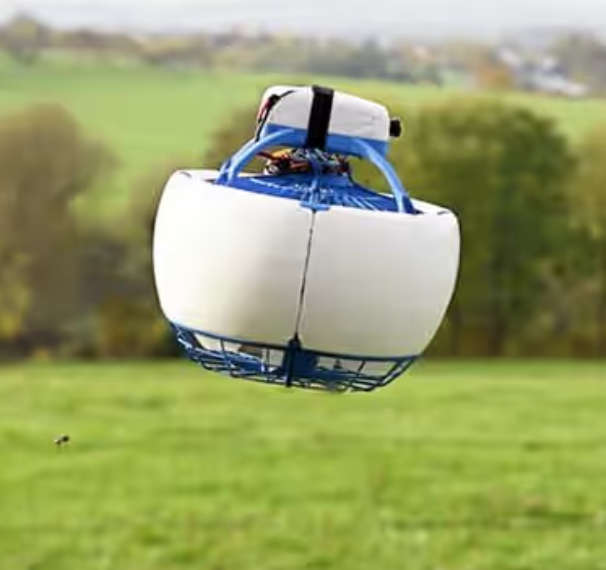
\includegraphics[width=5cm,height=5cm]{Fig/Fleye.png}
		\caption{\label{Fleye}Fleye}
	\end{minipage}%
	\begin{minipage}[c]{0.33\textwidth}
		\centering
		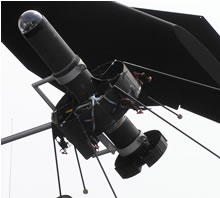
\includegraphics[width=5cm,height=5cm]{Fig/FanTail.png}
		\caption{\label{FanTail}FanTail}
	\end{minipage}
    \begin{minipage}[c]{0.33\textwidth}
		\centering
		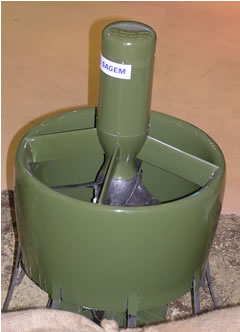
\includegraphics[width=4cm,height=5cm]{Fig/odin.jpg}
		\caption{\label{odin}Odin}
	\end{minipage}
\end{figure}

相较于国外的研究成果,我国DFUAV研究起步相对较晚,大多处于实验探索阶段。2008年,哈尔滨盛世特种飞行器有限公司与中国航天科工集团第四研究院和哈尔滨工业大学航天学院合作共同研发制造出国内首例单桨环道“飞碟”,直径1.2m,续航40分钟,最大速度可达80km/h,并获得国家发明专利。由南昌航空大学设计的“都市精灵”涵道无人机获得2011年“中航工业杯—国际无人飞行器创新大奖赛”创意奖,其涵道直径1.2m,续航时间1h,最大飞行速度为50km/h。深圳千叶智能科技公司以研发涵道式无人机设计平台为主,目前已推出CDF-270、CDF-390和EDF-254等型号的无人机,可用于航拍、巡航和侦察等领域。

\begin{figure}[htbp]
	\centering
	\begin{minipage}[c]{0.33\textwidth} % minipage将页面划分为0.5\textwidth
		\centering
		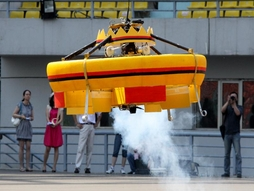
\includegraphics[width=5cm,height=5cm]{Fig/飞碟.jpg}
		\caption{\label{飞碟}飞碟}
	\end{minipage}%
	\begin{minipage}[c]{0.33\textwidth}
		\centering
		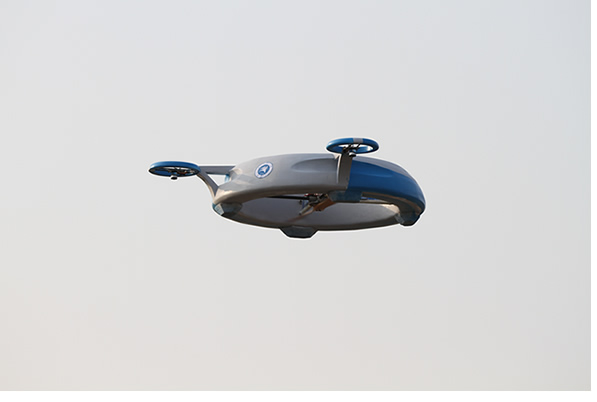
\includegraphics[width=5cm,height=5cm]{Fig/都市精灵.jpg}
		\caption{\label{都市精灵}都市精灵}
	\end{minipage}
    \begin{minipage}[c]{0.33\textwidth}
		\centering
		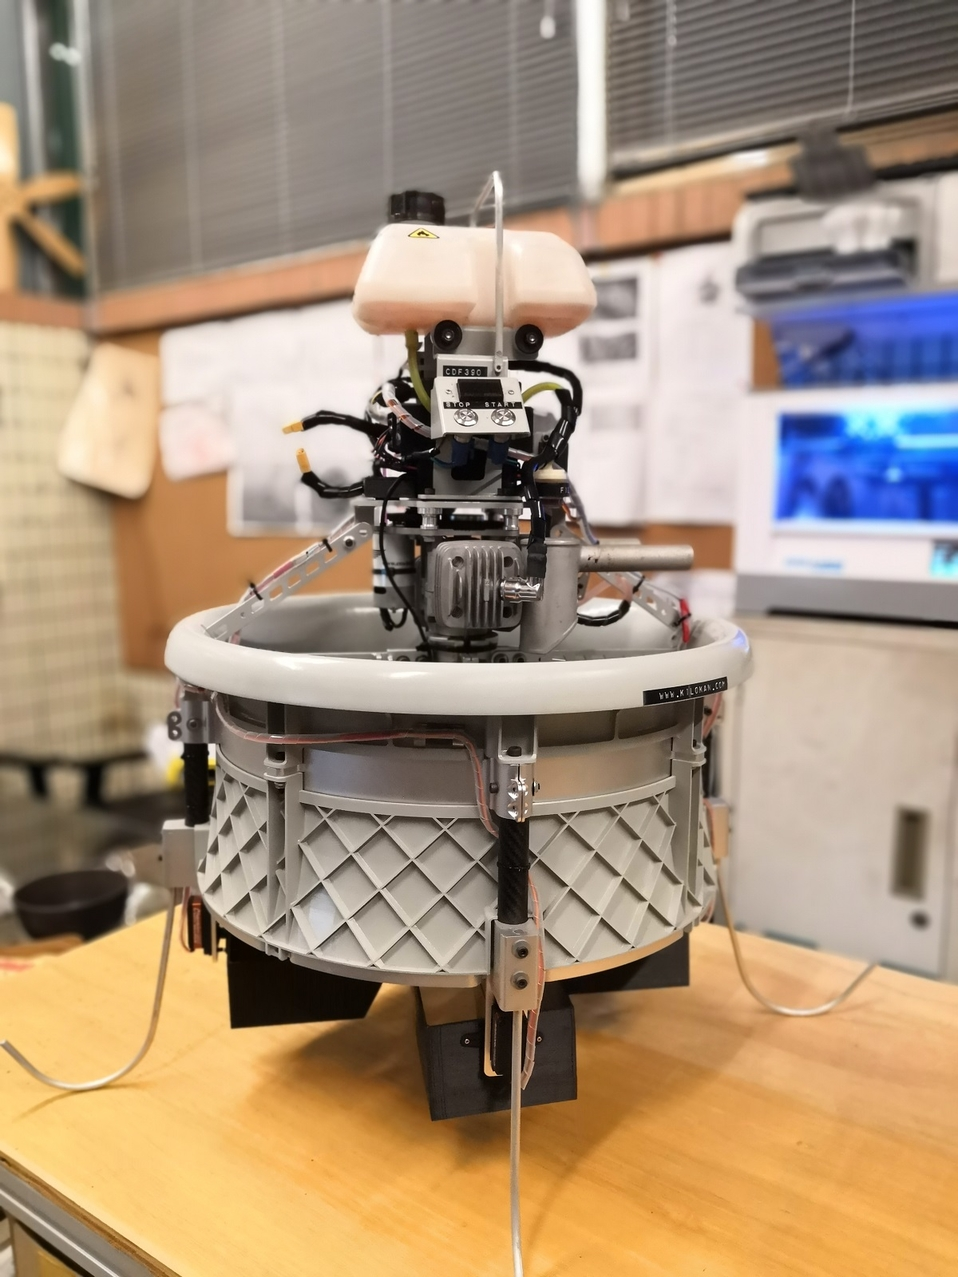
\includegraphics[width=4cm,height=5cm]{Fig/CDF-390.jpg}
		\caption{\label{CDF-390}CDF-390}
	\end{minipage}
\end{figure}

此外,清华大学\cite{chouStudyOverallDesign2021,luoNumericalAnalysisWind2024a}、北京理工大学\cite{manzoorCompoundLearningBasedModel2024}、南京航空航天大学\cite{caiNumericalPredictionUnsteady2022}和华南理工大学\cite{yinDuctedFanUAV2024,1022766347.nh}等高校也对DFUAV展开了不同程度的研究,极大推动了我国在该领域的发展进程。

\subsection{飞行控制技术}

无人机的飞行控制技术是其研究过程中的关键环节,其好坏直接影响了无人机的飞行性能和稳定性。在DFUAV发展的早期,由于对涵道风扇的独特气动特性认识不足以及控制理论体系的相对不成熟,DFUAV的控制器设计主要基于线性控制方法,如PID控制器、LQR控制器和$H_{\infty}$控制等。

上文提到的iSTAR微型DFUAV在2000年11月首次自由飞行时采用的就是PID姿态控制策略\cite{lipera2001micro}。为了实现位置控制,文献\parencite{erikssonPerformanceEstimationDucted2006}将整个控制系统分为外部和内部两个独立的子系统,采用串级PID方法进行控制,并且还实现了用于整个系统的LQ补偿器。Pflimlin等人早期在DFUAV的控制方面进行了深入研究\cite{pflimlinAerodynamicModelingPractical2007,pflimlinModelingAttitudeControl2010a},通过对悬停飞行条件线性化,简化飞行动力学,采用PID控制方法取得了较好的姿态跟随效果。2005年,他们推广了线性串级PID控制方法,提出了一种自适应反步控制策略着重于解决DFUAV在持续恒风条件下的稳定性问题,最后进行了仿真实验\cite{pflimlinPositionControlDucted2007b}。文献\parencite{whiteStabilityAugmentationFree}将LQR控制器与经典控制器相结合,通过时间响应和奇异值分析来评估控制系统的性能,实际飞行数据验证了该方法的有效性。文献\parencite{muehlebachFlyingPlatformTestbed2017}同样将LQR控制方法应用于DFUAV,该控制器具有级联结构,UAV的角速度由板载陀螺仪测量得到,位置、速度和姿态由外部的动作捕捉系统提供,最终通过实践证明了其可靠性。在$H_{\infty}$控制器的应用相关文献中,文献\parencite{DJKZ201009016}针对DFUAV易受干扰的特性设计了基于$H_{\infty}$理论的鲁棒控制器,通过仿真和实际飞行实验证明了该算法相比传统PID控制抗干扰性更强。文献\parencite{fanModellingAttitudeController2018}采用基于$H_{\infty}$合成的结构化多环反馈姿态控制器,并使用非光滑优化方法直接调节控制器参数到最优,确保了满意的实际控制效果。

虽然线性控制器易于实现,并且计算资源耗费较少,但是其性能往往受到系统的固有特性的限制,仅能够达到相对保守的性能\cite{manzoor2022flight}。当DFUAV由悬停转向高速飞行中应用线性控制器时\cite{saeedSurveyHybridUnmanned2018},控制性能会下降。作为替代,基于模型的非线性控制方法被广泛使用。如模型预测控制(MPC)、自适应控制和自抗扰控制(ADRC)等。

学者Tayyab Manzoor等人在DFUAV的MPC控制器设计上做了大量研究。在前期的工作中,他提出了一种无偏移的MPC框架来应对DFUAV的轨迹跟踪问题\cite{manzoorTrajectoryTrackingControl2020},控制策略分为内环和外环,两者都通过无偏移的MPC和卡尔曼滤波(KF)的组合来稳定跟踪。后来,为了飞行过程的鲁棒性能,又提出了一种将MPC与非线性干扰观测器结合的复合飞行控制技术\cite{manzoorMPCBasedCompound2020,manzoorCompositeObserverbasedRobust2023},并保证了闭环系统的稳定性。近年来,Tayyab Manzoor将ML与MPC相结合,提出基于复合学习的DFUAV的MPC方法\cite{manzoorModelPredictiveControl2023,manzoorCompoundLearningBasedModel2024}。该方法通过离线获取DFUAV的名义模型,在线使用强化学习优化控制策略,然后通过MPC进行优化和更新,提高计算效率,最后通过仿真证明了可行性。文献\parencite{zhaoModellingAttitudeControl2015}采用基于解耦的强自适应姿态控制方案,非线性的DFUAV在修整点进行了线性化,提升了系统的稳定裕度,仿真和实际飞行实验都表明姿态跟踪误差有效减少。文献\parencite{aiRobustAdaptiveControl2025}提出了一种基于控制增强的模型参考自适应控制架构,通过在线性时不变控制输入的基础上叠加自适应控制输入,以实时补偿不确定性,确保准确跟踪参考系统。实验表明该方法相比基线控制,速度跟踪误差减小了约38\%。文献\parencite{wenResearchVerticalTakeoff2021}介绍了该实验室设计的可变结构的垂直起降飞行器,基于动态模型进行解耦设计,并设计了一种离散的ADRC方法来控制其垂直起降过程。文献\parencite{yinDuctedFanUAV2024}使用ADRC控制器控制共轴双桨涵道无人机的姿态,使用固定于涵道壁的电磁铁来抓取物品,控制器用于抵消抓取过程中由于重量改变而引起的干扰,最终通过实际飞行实验表明无人机在抓取多个物品后依然能稳定姿态。

基于模型的非线性控制方法需要对系统模型有较为清楚的认识。除了基于模型的控制方法外,还可以采用基于传感器的方法:增量式非线性动态逆(Incremental Nonlinear Dynamic Inversion,INDI)。INDI作为一种重新配置的非线性动态逆(Nonlinear Dynamic Inversion,NDI)方法\cite{baconReconfigurableNDIController2001b,grondmanDesignFlightTesting},相比于NDI,对机载模型的依赖较小,并且只需要控制导数。在不确定的干扰情况下,气动变化会导致力与力矩的变化,而这些变化可以使用机载传感器测量得到,通过增量控制帮助系统快速稳定。Smeur等人对INDI控制技术进行了深入研究\cite{smeurAdaptiveIncrementalNonlinear2015,smeurCascadedIncrementalNonlinear2018b,steffensenNonlinearDynamicInversion2023},并成功在四旋翼无人机上进行应用。在文献\parencite{smeurAdaptiveIncrementalNonlinear2015}中,仅知道非常粗略的飞行器模型的情况下,使用自适应INDI控制器在线估计控制效果,最终在姿态控制方面表现出优异的抗干扰和自适应特性。文献\parencite{smeurCascadedIncrementalNonlinear2018b}中,该团队介绍了微型飞行器姿态控制的INDI和位置控制的INDI的串级结构,使用四旋翼进出10m/s的风洞,相比与PID控制情况下,位置误差显著减小。其他的应用包括垂直起降UAV的飞行过渡控制\cite{chengCorridorbasedFlightMode2023},轨迹跟踪控制\cite{taherinezhadEnhancedIncrementalNonlinear2023a}等。

此外,DFUAV的控制舵面通常装配冗余,控制输入的数量超过了系统自由度的数量,这导致了UAV的控制分配问题\cite{naldiPrototypeDuctedFanAerial2014b}。为了达到期望的控制效果,目前广泛采用的控制分配方法是伪逆法\cite{peddlePracticalHoverFlight2009a,pflimlinPositionControlDucted2007b,shengNearHoverAdaptiveAttitude2015b},直接计算从控制舵面角度映射到控制力矩的非方阵的伪逆矩阵。然而,由于实际的舵面角度受到约束,在伪逆操作下无法得到整个可达到的力矩的集合\cite{durhamAircraftControlAllocation2017a},导致在飞行包络线附近损失了舵面的部分控制能力\cite{HKXB202010026}。

\subsection{轨迹规划技术}

当飞行控制技术发展到一定阶段后,为满足更加多样化、个性化的飞行任务需求,以及应对充满不确定性、受各种约束情况下的飞行环境,对UAV的轨迹规划技术的研究也必不可少。一般情况下,轨迹规划过程分为两个部分:路径规划和轨迹优化。路径规划是指在给定的环境中,希望能够找到一条飞行路线,这条路线满足不与障碍物碰撞或者尽可能远离障碍物,并且满足路线最短等要求。而轨迹优化是对找到的飞行路线进行平滑处理并且赋予时间、速度等信息并且需要满足UAV的动力学约束。

在路径规划方面,目前广泛采用的方法主要有三类:
\begin{enumerate}[topsep = 0 pt, itemsep= 0 pt, parsep=0pt, partopsep=0pt, leftmargin=44pt, itemindent=0pt, labelsep=6pt, label=(\arabic*)]
	\item 基于栅格图的方法,该方法将待规划的环境划分为若干栅格,为栅格添加特殊标记以表示起点、终点、障碍物等信息。然后通过搜索算法如A*算法、D*算法、LPA*算法等在栅格中寻找一条最优路径。1968年,Hart等人提出了A*算法\cite{hartFormalBasisHeuristic1968},该算法通过引入与目标点有关的启发式信息,引导算法沿着最优路径前进。近年来,在A*算法的基础上出现了很多改进版本并成功应用于UAV的路径规划。文献\cite{liImprovedASTARAlgorithm2024}通过设置最小步长、最大倾斜角以及引入惩罚函数等方式来改造A*算法中的代价函数以适应UAV的飞行特性。实验结果表明改进后的算法相比改进之前减少了34.1\%的转弯角度,使得UAV飞行过程更加平稳,但是算法的扩展节点有所增加,耗时更久。D*算法由A*算法发展而来,D即Dynamic,相比于A*算法增加了动态避障搜索环节,主要用于机器人的自主寻路。Kadry等人通过在机器人移动过程中使用旋转矩阵的方式来改变机器人朝向,可以在某些情况下沿着弧线移动,进而能够更快的执行任务\cite{kadryPathOptimizationDstar2022}。
	\item 基于拓扑图的方法将环境表示为一个图,图中的节点代表环境中的位置,边则表示节点之间的连接关系。常用Dijkstra\cite{dijkstraNoteTwoProblems2022}算法和Floyd算法\cite{floyd1962algorithm}求解两点间最短路径。Dijkstra算法基于贪心策略,确保每次处理的节点都是距离起点最近的点,并且会判断更新到相邻节点的最短路径。文献\cite{zhuNewAlgorithmBased2021}在传统Dijkstra算法的基础上结合广度优先搜索、堆栈和队列数据结构提出了一种反向标记Dijkstra算法,通过理论分析得出该方法具有较低的时间复杂度,并且收敛速度优于常规算法。Floyd算法是在求解过程中将每个点轮流作为起点,重复执行多次Dijkstra算法,适合计算所有节点对之间的最短距离。由于包含了三重循环,所以时间复杂度较高,尤其是在处理稀疏图的情况下。
	\item 基于采样的方法包括概率路线图(PRM)\cite{geraertsComparativeStudyProbabilistic2004}、快速扩展随机树(RRT)\cite{lavalleRandomizedKinodynamicPlanning2001}以及一系列改进版本。无论是基于栅格图还是拓扑图的搜索都有一个前提就是需要对环境有较为清晰的认识,但当环境空间复杂或者维度高时,时间复杂度通常以指数增长,而基于采样的方法能够有效避免这一问题。PRM算法分为两步,首先在自由空间中生成多个点构成无碰撞的无向图,然后采用图搜索方法如Dijkstra来搜索从起点到终点的最优路径。但搜索的路径往往并非最优,所以有学者通过优化点的生成,去除冗余采样点和优化碰撞检测等方式改进路径质量\cite{liSmartVehiclePath2022}。RRT算法通过构建一颗以起点为根节点的随机树,逐步扩展,直到搜索到目标,因此RRT是一种增量式的搜索算法。但RRT同样有路径非最优的问题,因此有学者又提出了RRT*算法,通过在生成新节点后有条件地重构树节点,使得路径更加接近最优,但也因此耗费了时间。文献\parencite{fusicImprovedRRTAlgorithmBased2024}介绍了一种改进的RRT*算法,通过采用三角不等式重布线的方式来寻找UAV在三维环境下的无碰撞路径,仿真结果表明在时间和距离上相比RRT*更优。
\end{enumerate}

路径规划得到的飞行路线已满足无碰撞且尽可能距离最优,但往往不够平滑,不满足UAV的动力学约束。因此需要进行轨迹优化使路径平滑且满足动力学约束。最常用的轨迹优化方法是基于参数曲线的方法,如多项式曲线、贝塞尔曲线、B样条曲线、三次样条曲线等。基于参数曲线的方法优化的路径不仅仅是位置的平滑,更多的还包括速度、加速度乃至加加速度的连续,这一点对UAV的飞行至关重要。基于多项式曲线的轨迹优化是指参数$y$(如路径长度、速度)是参数$x$(如时间、曲率)的$n$次多项式。通过边界条件如起点、途径点和终点的位置以及速度、加速度等信息来确定多项式系数,从而得到平滑轨迹。文献\cite{arshadQuadrotorPathPlanning2023}中,在使用RRT*得到四旋翼的初步路径后,用多项式曲线表示了实际轨迹。1962年,法国工程师Bézier发现了一种用很少控制点就能得到复杂平滑曲线的方法,即贝塞尔曲线。但是在目前的实际应用中,用的最广泛的轨迹优化方法还是B样条曲线,B样条曲线由贝塞尔曲线发展而来,不仅保留了贝塞尔曲线的优点,还具备局部控制性质。文献\parencite{huangResearchPathPlanning2022,eshtehardianContinuousRRTbasedPath2023,fengSmoothPathPlanning2024a}都使用B样条曲线来表示最终轨迹。为了避免高阶多项式拟合过程中的龙格现象,使用多段样条曲线对型值点插值也是常用方法。可以通过相邻节点函数值相等、导数相等以及边界等条件来确定样条曲线的系数。文献\parencite{coteComplex3DFlighta}给出了一种基于三维三次样条曲线的完整轨迹方案。除基于参数曲线的轨迹优化方法外,还有二次规划方法\cite{arshadQuadrotorPathPlanning2023}、粒子群算法\cite{shinUAVPathPlanning2020}、人工势场法\cite{sunUavPathPlanning2022}等。

综上所述,轨迹规划方法种类繁多,每种方法都有自己的特点和适用场景,尽管有些方法一开始并非针对UAV的规划而提出,但在具体实践过程中依然可以根据彼此的特点和需求来选择合适的规划方法。

\section{本文的主要内容及章节安排}

本文针对DFUAV进行控制器设计以及轨迹规划设计,掌握被控对象的模型是基础,所以不可避免地需要首先对DFUAV进行数学建模分析。在此基础上,考虑到MPC控制器需要较高算力,ADRC控制器对参数较为敏感以及无法足够详尽的了解DFUAV的模型知识等情况,本文采用基于传感器的非线性控制方法:INDI控制。在优化控制分配问题方面,将参考文献\parencite{HKXB202010026}采用优先级控制分配(Priority Control Allocation,PCA)方案。最终实现基于INDI+PCA的DFUAV的姿态控制方案设计。然后,将INDI的理论思想扩展到速度环,实现速度、位置跟踪控制。在轨迹规划设计方面,考虑到DFUAV未来面临复杂多变的应用场景,因此本文采用基于采样的路径规划方法,结合RRT*算法和RRT-Connect算法各自的优势,提出C-RRT*算法。然后通过B样条曲线对路径进行平滑优化,最终实现DFUAV的自主飞行。

根据以上主要内容,本文的章节安排如下:

第一章:绪论。首先介绍了DFUAV的研究背景和意义,然后对DFUAV的国内外发展现状进行了概述,并且论述了DFUAV的飞行控制技术和轨迹规划技术的理论及应用。最后介绍了本文的主要内容及章节安排。

第二章:涵道风扇式无人机的系统建模与硬件设计。首先定义了DFUAV的坐标系和姿态表示方法,然后采用牛顿-欧拉方法推导出DFUAV的刚体运动学模型和刚体动力学模型,并分析了作用在涵道上的力与力矩。%最后介绍了DFUAV的硬件设计,包括传感器、执行器等。

第三章:涵道风扇式无人机的姿态控制。首先介绍了INDI控制器的基本原理,然后根据原理将INDI方法应用于姿态环。在底层的控制分配环节,采用PCA控制分配方法优先满足期望力矩。最后进行仿真和飞行实验,分析验证姿态控制器的性能。

第四章:涵道风扇式无人机的速度控制。根据INDI的理论思想将该方法扩展到速度环,实现速度、位置跟踪控制。最后进行仿真和飞行实验,分析验证速度控制器的性能。

第五章:涵道风扇式无人机的轨迹规划设计。首先介绍了RRT*算法和RRT-Connect算法的基本原理,结合两者的优势提出了C-RRT*算法。然后介绍B样条曲线的基本原理及性质,通过B样条曲线对C-RRT*算法搜索得到的路径进行平滑优化,最后进行实验验证。

第六章:总结与展望。首先对全文进行系统性地总结,分析了本文的创新点和不足之处,并对DFUAV未来的研究方向进行了展望。

